\documentclass[a4paper,12pt]{report}
\usepackage[utf8]{inputenc}
\usepackage[sfdefault]{roboto}

\usepackage{titling}
\usepackage{graphicx}
\usepackage{wrapfig}
\usepackage{subcaption}
\usepackage{float}
\usepackage{fontawesome}
\usepackage{setspace}
\usepackage[export]{adjustbox}
\usepackage[margin=20mm]{geometry}

\usepackage{xcolor}
\definecolor{turbo_purple}{RGB}{112,105,160}
\definecolor{sponsor_bronze}{RGB}{205,127,50}
\definecolor{sponsor_silver}{RGB}{170,169,173}
\definecolor{sponsor_gold}{RGB}{212,175,55}

\usepackage{titlesec}
\titleformat{\section}[block]{\normalfont\huge\bfseries\centering}{}{1em}{}
\titleformat{\subsection}[display]{\normalfont\Large\bfseries\color{turbo_purple}}{}{1em}{}
\titleformat{\subsubsection}[display]{\normalfont\large\bfseries}{}{}{\vspace{-1.2em}}[\vspace{-0.9em}]

\usepackage{fancyhdr}
\pagestyle{fancy}
\usepackage{tikz}
\usetikzlibrary{calc}
\usepackage{tikzpagenodes}
\fancyfoot{}
\renewcommand{\headrulewidth}{0pt}
\setlength{\headheight}{25pt}
\rhead{\begin{tikzpicture}[remember picture,overlay]
\draw  let \p1=($(current page.north)-(current page header area.south)$),
      \n1={veclen(\x1,\y1)} in
node [inner sep=0,outer sep=0,below left] 
      at (current page.north east){
\includegraphics[height=\n1]{Assets/Sponsorship Header - Solid.png}};
\end{tikzpicture}}
\lfoot{\begin{tikzpicture}[remember picture,overlay]
\draw  let \p1=($(current page footer area.north)-(current page.south)$),
      \n1={veclen(\x1,\y1)} in
node [inner sep=0,outer sep=0,above right] 
      at (current page.south west){
\includegraphics[height=\n1]{Assets/Sponsorship Footer - Solid.png}};
\end{tikzpicture}}
\cfoot{\sffamily\selectfont\thepage}

\usepackage[hidelinks]{hyperref}
\hypersetup{colorlinks=false}

\begin{document}

\begin{titlepage}
    \newgeometry{right=0mm,left=0mm,top=20mm,bottom=0mm}
    \begin{center}
        \vspace*{15mm}
        
\includegraphics[width=0.7\paperwidth]{Assets/Logo (Dark).png} \\
        \vspace{1cm}
        \Huge Sponsorship Prospectus \\
        \huge \textcolor{turbo_purple}{2023}
    \end{center}
    \vfill
    
\includegraphics[height=0.5\paperheight, right]{Assets/Pattern - PCB (Solid).png}
    \vspace*{10mm}
\end{titlepage}
\restoregeometry

\section*{About UQ MARS}
\subsection*{Who Are We?}

\begin{wrapfigure}{r}{0.4\textwidth}
\raisebox{0pt}[\dimexpr\height-\baselineskip\relax]{
    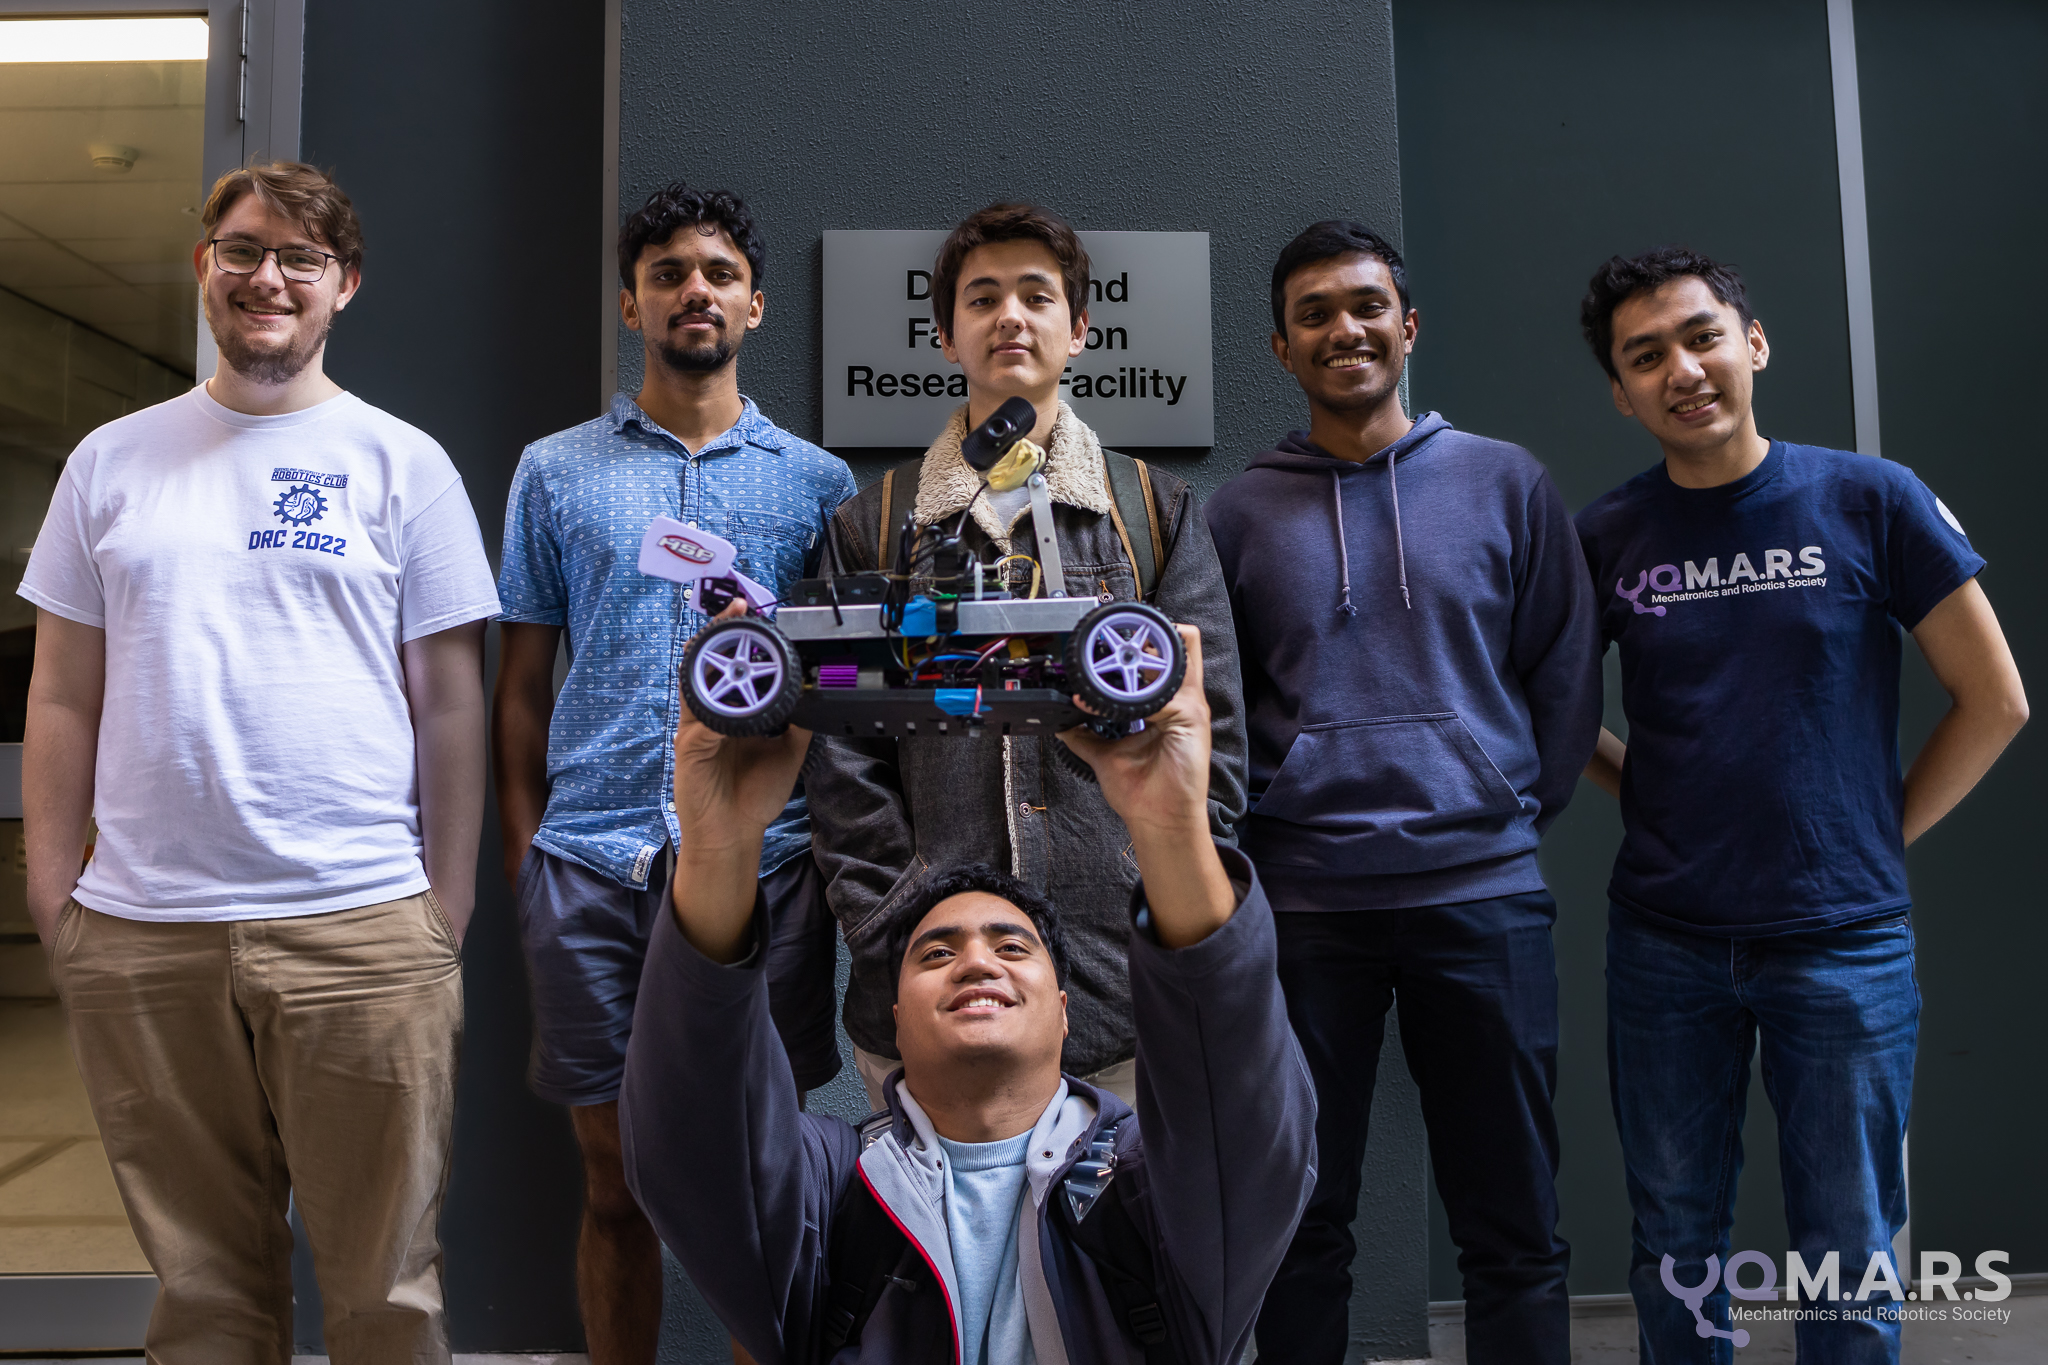
\includegraphics[width=0.9\linewidth]{Photos/DRC.jpg}
}
\end{wrapfigure}

The UQ Mechatronics and Robotics Society is a student-led hub for passion and innovation in robotics and automation.
Connecting members across disciplines and year levels, the society aims to foster a strong community centered on the practical development of robotics.
Aspiring engineers have the opportunity to connect through our hosted workshops, seminars and competition teams.

\subsection*{What Have We Achieved?}
In 2022, UQMARS saw massive success, through a variety of events, collaborations, and an increase in membership numbers more than triple to 161 when compared to 2021 (with an average of approximately 20\% attendance at each event).
Some of our notable events in 2022 include:
\begin{itemize}
    \item \subsubsection{Big Fat Small Clubs Launch Party}
    In collaboration with 15 other UQ clubs and societies, we hosted a social launch event designed to help ease members into the first semester.
    The event served as an opportunity for students from all disciplines to meet and connect as university was beginning for the year.
    \item \subsubsection{Mechatronics Information Night}
    This event was a collaboration with both Engineers Without Borders and Robogals and was designed to introduce members to applications of a mechatronic engineering degree, particularly through a humanitarian lens.
    The evening featured professionals both from education and industry backgrounds to inspire members with their own experiences.
    \item \subsubsection{Arduino Hackathon}
    The Arduino Hackathon was a three-day event held in collaboration with QUT Robotics Club and Robogals, with a theme of ‘assistive technology’.
    The event served as an opportunity for members to test their abilities and develop new skills around developing with embedded systems.
    \item \subsubsection{Droid Race Competition}
    In 2022, UQ MARS entered two teams into the QUT Droid Race Challenge.
    The competition presents an opportunity for members to get hands-on experience with computer vision, control systems, and mechanical design.
    Teams performed admirably, with both managing to outperform the hosts.
    \item \subsubsection{Torch Workshop Series}
    One of our largest attractions for the year was a seven part torch building workshop series. This series taught members various skills in mechatronics, including circuit board design, soldering skills, CAD design and more.
\end{itemize}

\newpage

\section*{UQ MARS in 2023}
\subsection*{Goals}
Looking ahead to 2023, UQ MARS is focused on building on past achievements as a foundation from which we can grow. Our priorities moving forward are to:
\begin{itemize}
    \item Continue to increase membership and engagement
    \item Provide more opportunities for members to develop essential mechatronics skills
    \item Build industry connections and collaborations
    \item Drive the social culture around the club
    \item Give back to our community
\end{itemize}

\begin{figure}[H]
    \centering
    \begin{subfigure}{0.32\linewidth}
        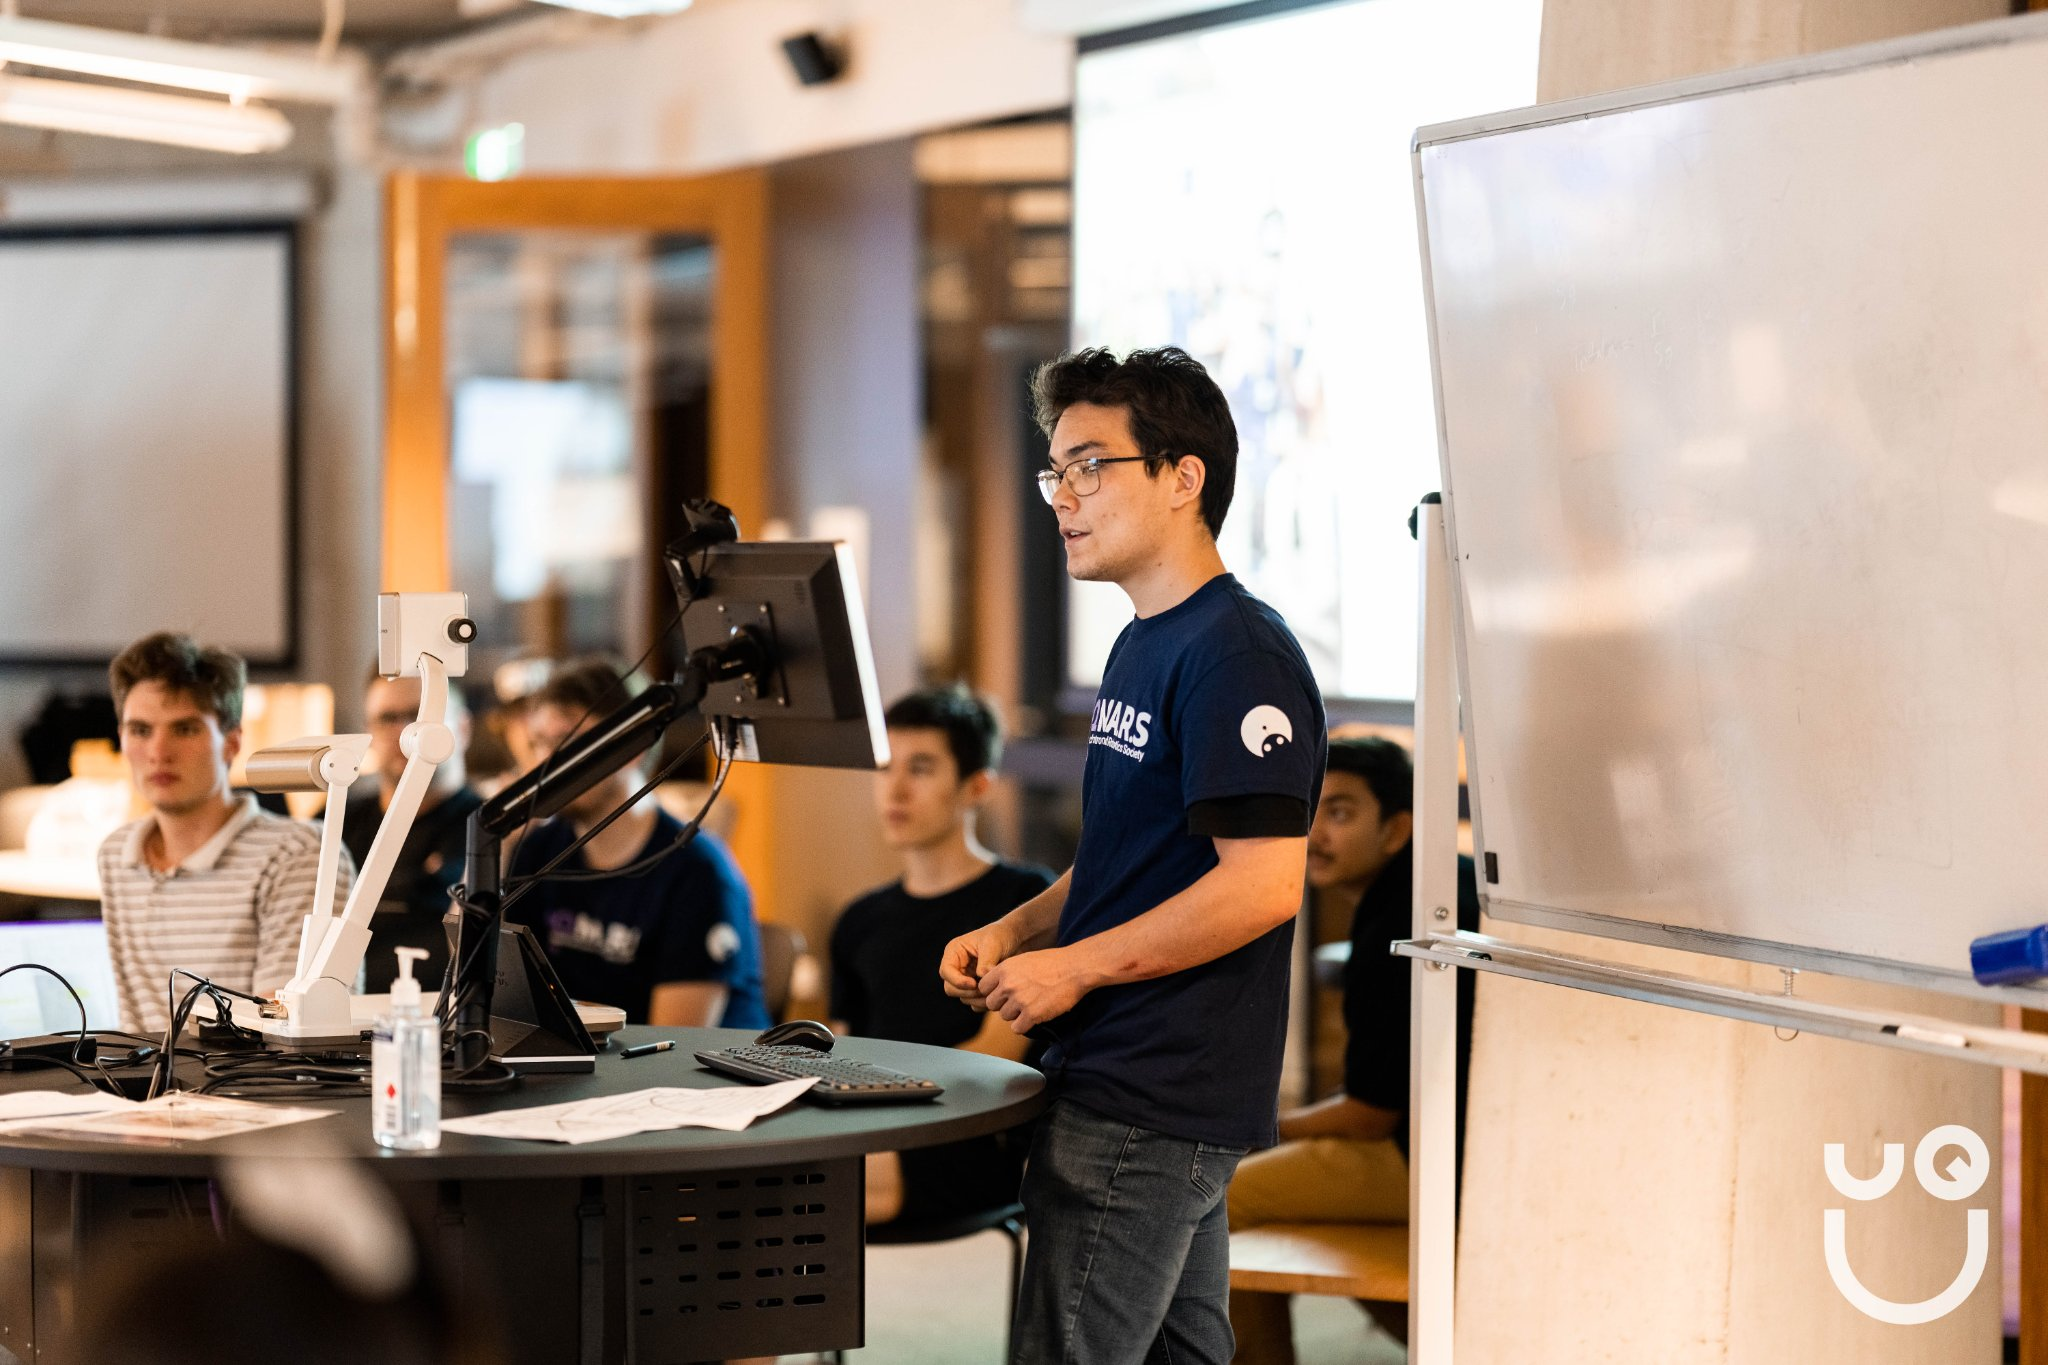
\includegraphics[width=0.99\linewidth]{Photos/Hackathon.jpg}
    \end{subfigure}
    \begin{subfigure}{0.32\linewidth}
        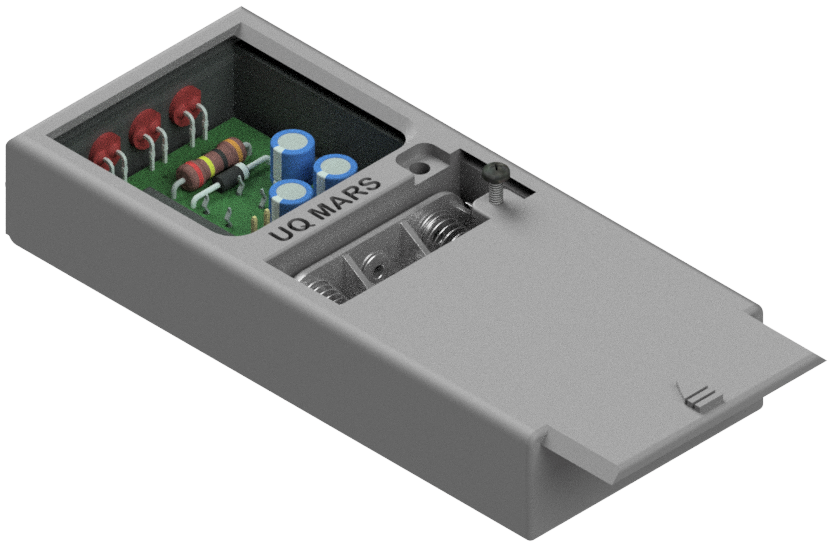
\includegraphics[width=0.99\linewidth]{Photos/Torch.png}
    \end{subfigure}
    \begin{subfigure}{0.32\linewidth}
        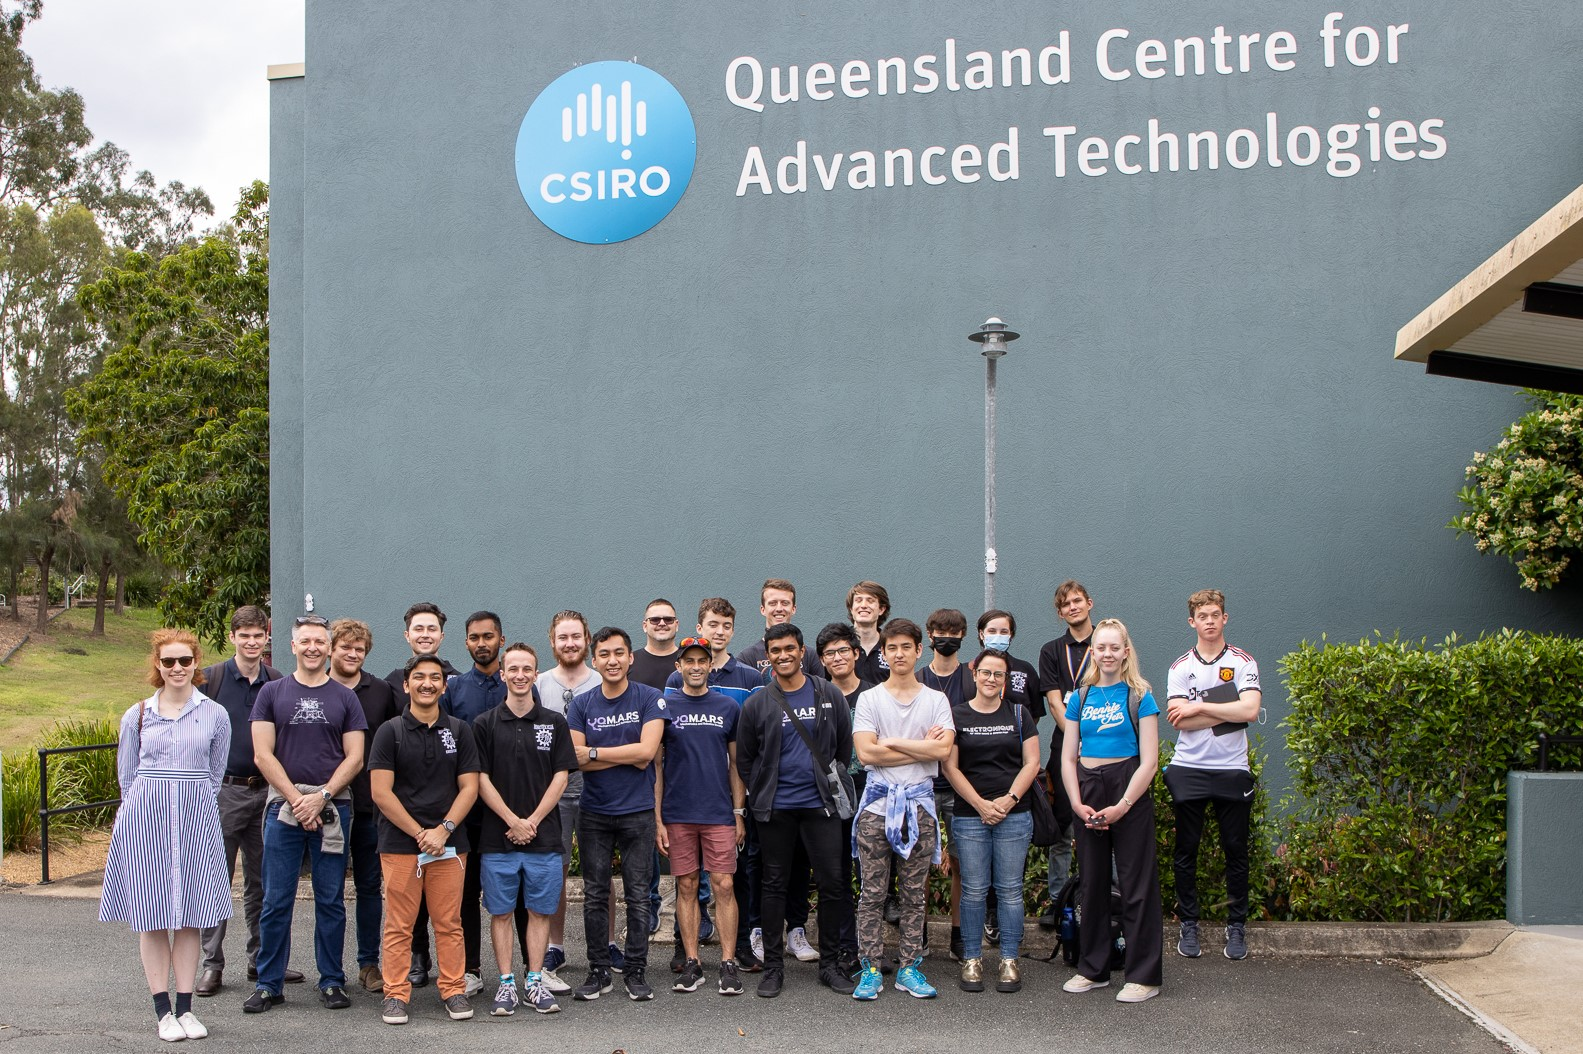
\includegraphics[width=0.99\linewidth]{Photos/CSIRO.jpg}
    \end{subfigure}
\end{figure}

\subsection*{Micromouse Competition}
The micromouse competition sees competitors design a small robot to solve a $N\times N$ maze in the fastest time possible.
This compels competitors to utilise the best algorithms and design the fastest robot mice possible. We aim to host this competition in UQ Innovate and live-stream it through our YouTube channel.
There will be three main challenges:
\begin{itemize}
    \item Fastest time
    \item Cheapest design
    \item Going over correct checkpoints and avoiding others
\end{itemize}
While the \textit{cheapest design} challenge can be done in tandem, the other two challenges will be separate races. We believe these three challenges will produce unique designs and all some flavour to a competition first held in the 1970`s.

To ensure that our competition is up to international standards, we are in contact with IEEE, Techfest, UK Micromouse and Robotics Society, and Lunghwa University of Science and Technology. 

\newpage

\subsection*{Workshops}
Workshops have been at the heart of our society's events. They help our members gain skills they otherwise wouldn't for both professional and personal use.
Where possible, we will be recording our workshops and uploading them to our YouTube account for members' future reference.
\begin{itemize}
    \item \subsubsection*{UQ Innovate Training}
    Following student and member feedback that they wish to get more hands-on training with industrial tools and software, we will be running a series of training.
    Sessions for gaining said training. At UQ Innovate we will be running CNC laser-cutting, machining, and milling.
    \item \subsubsection*{PCB Design}
    We look forward to improving the PCB designing capabilities of our members and other students interested.
    The workshops will provide a step-by-step experience and foster an environment for students to learn how to use software used in the industry such as Altium.
    \item \subsubsection*{CAD Drawings}
    In 2023 we also aim to improve our member's skills using CAD software such as Autodesk AutoCAD or SIEMENS NX.
    These practicals will also provide a step-by-step process where students will design basic objects, to begin with, and slowly improve their skills.
    \item \subsubsection*{Microcontroller Utilisation}
    Understanding how to effectively choose a microcontroller fit for purpose and then programming it can be daunting for many students.
    We aim to teach students how to read microcontroller data-sheets so that they can better select one for their projects and program them using C/C++.
    \item \subsubsection*{Sensor Synthesis}
    To effectively control a system, students need to be able to read and record sensor data effectively so that their projects operate as intended.
    We will start by teaching students how different sensors work, then in a more advanced workshop, we will teach students how to develop sensor fusion algorithms using MATLAB Simulink modelling.
    \item \subsubsection*{Computer Vision}
    Computer vision workshops have been our most popular workshops.
    Each workshop has taught a different aspect of computer vision.
    This also serves as foundational knowledge for some of our competitive teams such as Droid Race Competition.
    \item \subsubsection*{Planning and Pathing Algorithms}
    Next year we plan to co-host two pathing and planning algorithm workshops with UQ Computing Society.
    The first will focus on commonly used pathing algoritmns and the second will teach students how to take different sensor information and use that to path plan.
    This workshop would be used as an introduction to our Micromouse competition.
\end{itemize}

\newpage

\subsection*{Arduino Hackathon}
Each year, we host a Hackathon in conjunction with Robogals and QUT Robotics.
The event starts with an introduction night, which allowed students the opportunity to network and form teams.
The event pushes for students to connect and form lasting relationships with students from other universities, and develop new skills around embedded technology through project-based learning with Arduinos (such as programming control systems in C++).
Each society will bring one sponsor to judge each team`s project. Each year there is a theme for students to use as a guide.
One outcome of this annual event, is to provide Robogals new material to teach at their workshops aimed at inspiring young women to join STEM.

\begin{figure}[H]
    \centering
    \includegraphics[width=0.9\linewidth]{Photos/Arduino1.jpg}
\end{figure}


\subsection*{Regular Talks and Seminars} 
As a means to introduce members to some of the more obscure and interesting applications of mechatronics and robotics, we plan to make our hosted talks and seminars a regular feature.
These events are presented by researchers, students and industry professionals in fields that they have experience / interest in.

\subsection*{Community Outreach}
We hope to inspire the engineers of tomorrow through outreach workshops intended to introduce current high school students to the fields of mechatronics and robotics.
We will involve members within the running of these workshops to help them with the development of their own interpersonal skills.

\subsection*{Inter-Society and Inter-University Events}
We understand that tertiary study is more than your classes, it's also the connections and friendships you make while undertaking study.
Next year, we are committed to building strong relationships with other student societies both at the University of Queensland and elsewhere.
As part of this commitment we will be running and hosting a '\textit{Show and Tell}' night for members of UQ STEM Societies to show of their personal projects.

\subsection*{Mechatronics Study Guide}
We are currently developing a comprehensive course guide to aid students in the selection of their courses.
The guide will present suggested program structures, enrolment plans, course profiles, and offer the chance to inform students of the specific pathways available within Mechatronics and adjacent specialisations such as Electrical/Computer Engineering.
We will aim to give specialised advice from our executive team and various UQ MARS Alumni regarding study advice, course selection and general career advice.

\begin{figure}[H]
    \centering
    \includegraphics[width=0.85\linewidth]{Photos/HardAF.jpg}
\end{figure}

\newpage

\section*{Sponsorship}
\large
We offer a number of sponsorship packages which are laid out below. The prices provided are annual figures, quoted in AUD.
\normalsize

\subsection*{
    
\includegraphics[width=1em]{Sponsor Icons/Bronze}
    \textcolor{sponsor_bronze}{Bronze Tier (\$500)}
}
Bronze Tier sponsorship will have you:
\begin{itemize}
    \item Listed on the club website
    \item Given the opportunity to promote intern and graduate positions to our members
\end{itemize}

\subsection*{
    
\includegraphics[width=1em]{Sponsor Icons/Silver}
    \textcolor{sponsor_silver}{Silver Tier (\$1000)}
}
Silver Tier sponsorship will include the perks of Bronze Tier, plus:
\begin{itemize}
    \item Listed in the Mechatronics course guide
\end{itemize}
And, the opportunity to either:
\begin{itemize}
    \item Present one of our regular talks / seminars; or,
    \item Send representation to one of our industry events (such as panels or networking nights)
\end{itemize}

\subsection*{
    
\includegraphics[width=1em]{Sponsor Icons/Gold}
    \textcolor{sponsor_gold}{Gold Tier (\$1500)}
}
Gold Tier sponsorship entitles you to all of the available perks of Silver Tier, plus:
\begin{itemize}
    \item Advertised in all workshop sessions
    \item Brand placement on our competitive team uniforms (worn for events like Droid Race Competition)
\end{itemize}

\subsection*{
    
\includegraphics[width=1em]{Sponsor Icons/Turbo.png}
    \textcolor{turbo_purple}{Turbo Tier (\$2000+)}
}
Turbo Tier sponsorship is our most comprehensive package, entitling you to all of the perks of Gold Tier, in addition to having your name on \textbf{one} of:
\begin{itemize}
    \item Arduino Hackathon (1 Slot)
    \item Droid Race Competition (3 Slots)
    \item Micromouse Competition (3 Slots)
    \item A dedicated section for your company within the Mechatronics course guide and other UQ MARS materials
\end{itemize}

\newpage

\section*{Contact Us}
\begin{figure}[H]
    \centering
    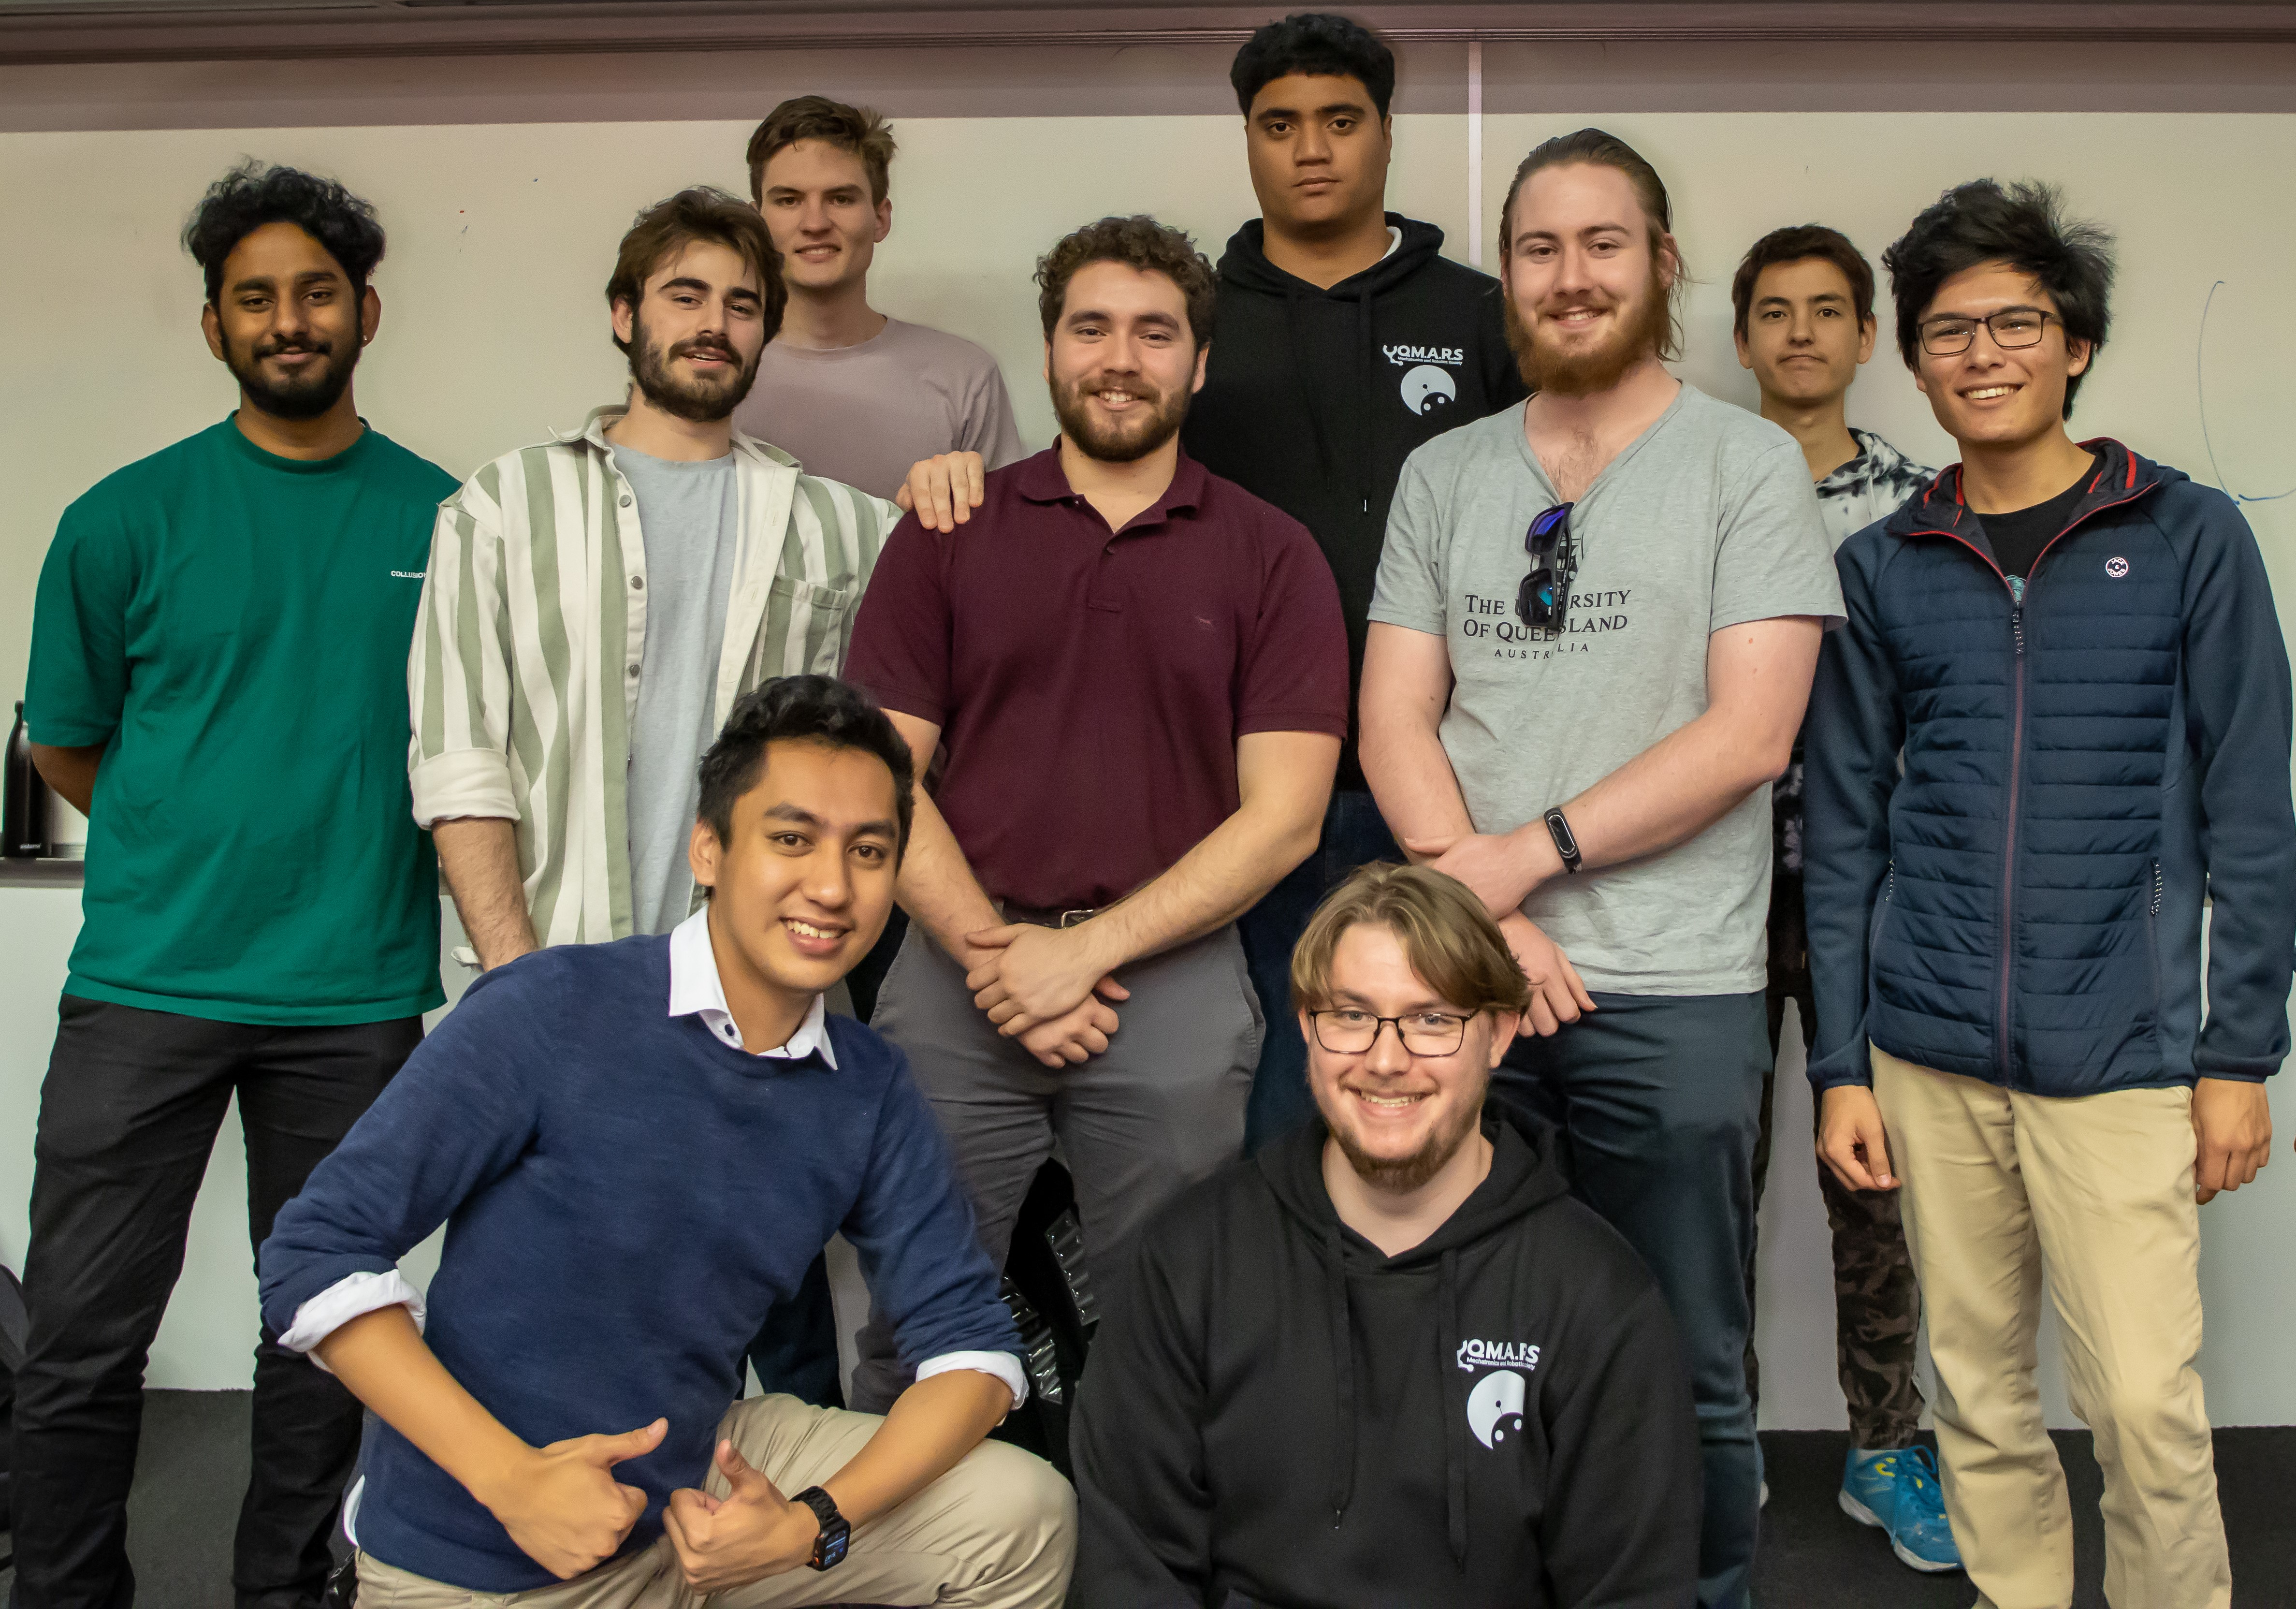
\includegraphics[width=0.9\linewidth]{Photos/Exec.jpg}
\end{figure}

\large
\onehalfspacing
You can contact us through any of the following platforms: \\
\faLink{} \href{https://www.uqmars.com}{uqmars.com} \\
\faEnvelope{} \href{mailto:uqrobotics@gmail.com}{uqrobotics@gmail.com} \\
\faFacebookSquare{} \href{https://facebook.com/UQMARS}{UQ MARS} \\
\faLinkedinSquare{} \href{https://linkedin.com/company/uq-mars}{UQ Mechatronics and Robotics Society (UQ MARS)} \\
\faGithubSquare{} \href{https://github.com/uqmars}{UQ Mechatronics And Robotics Society} \\
\faYoutubePlay{} \href{https://www.youtube.com/channel/UCH3GjoKLL3R_1ayjkn9C78A}{UQ MARS} \\
\faInstagram{} \href{https://www.instagram.com/uq.mars/}{uq.mars} \\
We look forward to hearing from you!

\end{document}
